\chapter{Applying $T_2$ Relaxation Under Spin Tagging (TRUST) To Assess Renal Oxygenation}
\label{chap:TRUST}

\begin{abstract}
	This work was presented as an aural presentation at the \ac{ISMRM} 26th Annual Meeting (2018) \cite{daniel_applying_2018}.\\
	
	\lipsum[1]
\end{abstract}
\newpage

\section{Introduction}
Sufferers of \ac{CKD} can have abnormalities in kidney structure or reduced urine function. More quantitively \ac{CKD} can be assessed clinically by \ac{GFR}, the rate at which fluid is filtered through the kidneys, with a value below 60 ml/min/1.73m$^2$ of body surface area being diagnostic or the presence of albumin, the main protein in blood plasma, in the patients urine \cite{stevens_assessing_2006, farrugia_albumin_2010, pruijm_blood_2017}. An estimated 5–11\% of the global population suffer from \ac{CKD} \cite{
	coresh_prevalence_2003, de_lusignan_identifying_2005, drey_population-based_2003, amato_prevalence_2005, chadban_prevalence_2003} making it a significant public health concern. Late referral of renal disorders results in an increase in mortality rate and treatment costs \cite{jungers_late_1993, sesso_late_1996, klebe_cost_2007}. Given that in 2013/2014 renal services cost the United Kingdom's National Health Service \pounds 586 million \cite{precious_nhs_2015} there are clear health and economic advantages to an early diagnosis of \ac{CKD}.\\

The current methods available for \ac{CKD} diagnosis are not ideal for a variety of reasons. Histological samples are the gold standard for diagnosis however collecting them is an invasive process and as such they are not suitable for monitoring the progress of a patient's condition on a regular basis. This coupled with the fact that a small sample is not representative of the entirety of both kidneys means that this method  has large drawbacks. Ultrasound can be used to gather structural information about the kidneys non-invasively, however, it suffers from low spatial resolution and the images being difficult to interpret. The most common method of diagnosis is to estimate \ac{GFR} from the creatinine content in a blood sample however this measure does not allow for the individual assessment of each kidney and is an indirect measure of kidney tissue damage.\\

\ac{MRI} is a flexible non-invasive tool that can be used to collect a wealth of information about the kidneys. A current research interest at the \ac{SPMIC} is to use multi-parametric renal \ac{MRI} to assess and predict \ac{CKD}. This protocol assesses haemodynamics, oxygenation and microstructure in a single 45 minute scanning session and shows significant changes in certain combinations of parameters in subjects with \ac{CKD} as opposed to healthy volunteers \cite{cox_multiparametric_2017}. Currently oxygenation is assessed using \ac{BOLD} $T_2^*$ maps to measure oxygenation of different tissues within the kidney, predominately the separation in mean $T_2^*$ between the renal cortex and medulla, an example of which is shown in Figure \ref{fig:T2*map}. These \ac{BOLD} $T_2^*$ maps are, however, affected by other factors such as susceptibility effects, shimming and baseline blood flow and thus may be limited in their ability to draw quantitative conclusions despite their widespread use \cite{pruijm_blood_2017, niendorf_how_nodate}. 
\begin{figure}[H]
	\centering
	\includegraphics[width=0.45\textwidth]{TRUST/T2star_map.eps}
	%\missingfigure{T2* Map}
	\caption{An example $T_2^*$ map. A clear difference can be seen between the renal medulla and cortex.}
	\label{fig:T2*map}	
\end{figure}

A welcome addition to this multi-parametric model would be the assessment of \ac{RMRO$_2$}; a measure analogous to the \ac{CMRO$_2$} \cite{chong_cerebral_2015}. This measure can be calculated via Equation \eqref{eq:RMR02}
\begin{equation}
\textup{RMRO}_{\textup{2}} = \left( Y_a - Y_v \right) \times \textup{RBF} \times \left[\textup{Hct}\right]
\label{eq:RMR02}
\end{equation}
where $Y_a$ and $Y_v$ are arterial and venous oxygen saturation respectively, RBF is renal blood flow (in ml/min) and Hct is the ratio of the volume of erythrocytes to the volume of the rest of the blood, known as haematocrit. \ac{RBF} can be measured relatively easily using \ac{PC}-\ac{MRI} \cite{jordan_velocity_1994} and Hct is usually taken to be 0.41 for healthy adults but can be measured from a simple blood test \cite{miao_reference_2002, gardener_dependence_2010} or using the correlation between $T_1$ of blood and its haematocrit \cite{shimada_vivo_2012}. This means that only a measurement of blood oxygen saturation via a non-invasive protocol is required to generate a quantitative value of \ac{RMRO$_2$}.\\

Blood oxygen saturation can be measured precisely via the insertion of catheters into the patient, however this is clearly an invasive process \cite{nagdyman_comparison_2005}. There are currently two well established methods of measuring blood oxygenation via \ac{MRI} however these have only been used in the brain thus far. These methods are \ac{TRUST} \cite{lu_quantitative_2008, xu_improving_2012, liu_testretest_2013, liu_multi-site_2016} and susceptibility-based oximetry \cite{jain_mri_2010, jain_cerebral_2014, driver_global_2014, lee_multiplexed_2017}. \ac{TRUST} builds on the ideas of an \ac{ASL} sequence in the fact that by subtracting control images from labelled images only blood is imaged. However, instead of labelling a slab of tissue in the neck and imaging a superior slice, when implementing \ac{TRUST} the imaging plane is inferior to the labelled slab. By collecting a series of pairs of labelled and control images with different $T_2$ weightings it is possible to fit the data from the sagittal sinus to a $T_2$ relaxation and use a calibration curve to convert the value of $T_2$ to venous oxygenation \cite{wright_estimating_1991}. Susceptibility-based oximetry is based upon the differences in magnetic susceptibility between the blood and the surrounding tissue. Using a phase map it is possible to model this difference in susceptibility and using the known difference in susceptibility between fully oxygenated blood and fully deoxygenated blood, venous oxygenation can be calculated.\\

Here both of the above techniques are applied to study oxygenation in the renal vein in young healthy individuals to assess the technicalities of transferring these protocols from the brain to the body. Given that these techniques have already been used in the brain with a number of studies in the literature, the sequences are first implemented on the brain to assess oxygenation in the superior sagittal sinus, then adapted to work within the more challenging environment of below the neck applications. These adapted sequences are compared to the results gained using the established techniques in the brain before testing on the renal vein. An oxygen challenge is carried out to verify that changes in oxygenation can be measured in the renal vein. If proved successful these sequences will be incorporated into the multi-parametric renal \ac{MRI} protocol.\\

\newpage
\section{Methods}

Imaging was performed on a whole body 3 Tesla \ac{MRI} scanner (Ingenia, Philips Medical Systems, The Netherlands) using a 32 channel head or body coil. Studies were carried out according to the principles of the Declaration of Helsinki and approved by either the Local Ethics Committee or the East Midlands Research Ethics Committee. Written informed consent was obtained from all subjects.\\

\subsection{Susceptibility-Based Oximetry}
\label{sec:SBO}
\subsubsection{\ac{MRI} Protocol}
\label{sec:SBO_prot}
The principle behind susceptibility-based oximetry is based on the fact that there is a difference in magnetic susceptibility between the blood within a vessel and the tissue surrounding it \cite{haacke_vivo_1997}. As outlined by Jain, if a blood vessel is modelled as a long paramagnetic cylinder, it is possible to calculate the oxygenation of the blood by knowing the phase difference between blood in the vessel and the surrounding tissue, the angle of the vessel to the $B_0$ field, the echo time of the scan and the subject's haematocrit \cite{jain_mri_2010}. This relationship is shown in Equation \eqref{eq:SBO}.
\begin{equation}
\textup{Y}_{\textup{v}} = \left[ 1-\frac{2|\Delta\phi|}{\gamma TE\Delta\chi_{\textup{do}}B_0(\cos^2\theta-1/3)\textup{Hct}}\right]\times 100
\label{eq:SBO}
\end{equation}
where $\Delta\phi$ is the average phase difference between the blood in the vessel and the surrounding tissue, $\gamma$ is the gyromagnetic ratio of a proton, TE is the echo time, $\Delta\chi_{\textup{do}}$ is the susceptibility difference between fully deoxygenated and fully oxygenated blood ($4\pi\times0.27\textup{p.p.m}$) \cite{spees_water_2001, jain_investigating_2012}, $B_0$ is the static field strength, $\theta$ is the angle of the vessel to the $B_0$ field and Hct is the subjects haematocrit. Given haematocrit can be assumed or is measured with a blood test or by measuring the $T_1$ of the blood, this means that from a simple phase map it is possible to calculate $Y_v$. The optimum phase map for this purpose was produced using a 2D $T_1$ weighted \ac{FFE} sequence with a flip angle of $25\degree$, flow compensation, coil homogeneity correction and flyback. The \ac{FOV} was 230$\times$184$\times$29 mm, matrix size of 400$\times$300, \ac{TR} of 12 ms, \ac{TE} of 7.5 ms and three signal averages. This led to a total acquisition time of 9 seconds and as such could be completed in a single breath hold if required.\\

\subsubsection{Analysis}

Once the phase map has been acquired, a \ac{ROI} containing the superior sagittal sinus was defined. This mask was then dilated with concentric shells to generate the two \ac{ROI} shown in Figure \ref{fig:SBO_ROI}, note that the outer \ac{ROI} has been constrained to within the brain during its dilation. There were no occurrences of phase wrapping in or immediately surrounding the superior sagittal sinus observed due to its small size and the high field homogeneity within the head and of the 3T scanner used. Any occurrences of phase wrapping could easily be corrected using \ac{PRELUDE}, a tool within \ac{FSL} (fMRIB, The University of Oxford) \cite{jenkinson_fast_2003}. The average values of phase within these two \ac{ROI} along with the angle of the vessel to the $B_0$ field, as calculated from the localisation scans can then be used with Equation \eqref{eq:SBO} to calculate $Y_v$.\\

\begin{figure}[H]
	\centering
	\includegraphics[width=0.6\textwidth]{TRUST/SBO_ROI}
	\caption{The region of interest averaged to find the intra-vascular phase (blue) and the region of interest used to find the phase of the surrounding tissue (red).}
	\label{fig:SBO_ROI}	
\end{figure}


\subsection{$T_2$ Relaxation Under Spin Tagging}

\subsubsection{\ac{MRI} Protocol}
\label{sec:TRUST_MRI}

The protocol for the \ac{TRUST} \ac{MRI} sequence in the brain involves the acquisition of a series of paired images using the pulse sequence shown in Figure \ref{fig:TRUST_TILT_Seq}. A series of presaturation pulses using the \ac{WET} scheme are applied to the imaging slice, shown in Figure \ref{fig:TRUST_Brain}, to reduce the signal from static tissue and reduce contamination of the magnetisation in the imaging slice by an imperfect labelling slab profile \cite{hendrikse_measurements_2003, golay_pulsed_2005}. In the first of each image pair, a labelling pulse is applied consisting of two successive slice-selective $90\degree$ \ac{RF} pulses to generate a $180\degree$ label. The next image in the sequence has a control pulse applied to it instead of a labelling pulse, in this image the second of the $90\degree$ pulses is applied $180\degree$ out of phase to give zero net effect. As such any effects of magnetisation transfer related signal in the stationary tissue can be cancelled out because the net \ac{RF} effect on the macromolecular spin magnetization is identical for both the labelling pulse and control pulse. This method of labelling is known as \ac{TILT} and is widely used in literature for labelling in \ac{TRUST} in the brain \cite{golay_transfer_1999}. A series of non-selective $T_2$ preparation pulses are then applied to minimise the blood outflow effect and modulate the $T_2$ weighting of the image, the time between the application of the labelling pulse and the $T_2$ preparation is known as the \ac{PLD}. Finally a $90\degree$ excitation pulse is applied followed by a standard \ac{EPI} readout at time \ac{TE} later \cite{xu_improving_2012}. If the control image is subtracted from the labelled image then only the venous blood that flowed from the labelled slab to the imaging slice will be visible, as shown in Figure \ref{fig:SS_labsub}.\\

\begin{figure}[H]
	\centering
	\begin{subfigure}[c]{1.0\textwidth}
		\centering
		\includegraphics[width=1\textwidth]{TRUST/TRUST_TILT.eps}
		\caption{}
		\label{fig:TRUST_TILT_Seq}
	\end{subfigure}
	\vskip\baselineskip
	\begin{subfigure}[c]{0.8\textwidth}
		\centering
		%\missingfigure{TRUST_TILT_Brain.ai from ISMRM presentation}
		\includegraphics[width=0.6\textwidth]{TRUST/TRUST_TILT_Brain.eps}
		\caption{}
		\label{fig:TRUST_Brain}
	\end{subfigure}
	\caption{(\subref{fig:TRUST_TILT_Seq}) The pulse sequence for \ac{TRUST} \ac{MRI} using the TILT labelling sequence. (\subref{fig:TRUST_Brain}) The labelling and imaging volumes used for TILT tagging within the brain.}
	\label{fig:TRUST_TILT}
\end{figure}
\newpage
\begin{figure}[H]
	\centering
	\begin{subfigure}[c]{0.30\textwidth}
		\centering
		\includegraphics[width=1\textwidth]{TRUST/Brain_Control}
		\caption{}
		\label{fig:SS_cont}
	\end{subfigure}
	\hfill
	\begin{subfigure}[c]{0.30\textwidth}
		\centering
		\includegraphics[width=1\textwidth]{TRUST/Brain_Label}
		\caption{}
		\label{fig:SS_lab}
	\end{subfigure}
	\hfill
	\begin{subfigure}[c]{0.30\textwidth}
		\centering
		\includegraphics[width=1\textwidth]{TRUST/Brain_eTE_1}
		\caption{}
		\label{fig:SS_diff}
	\end{subfigure}
	\caption{The control image, (\subref{fig:SS_cont}), is subtracted from the labelled image, (\subref{fig:SS_lab}), to generate  a difference image, (\subref{fig:SS_diff}), of only the tagged blood.}
	\label{fig:SS_labsub}
\end{figure}

This process is then repeated for another pair of images, however, this time the duration of the $T_2$ preparation is increased to a larger \ac{eTE}, this applies a $T_2$ weighting to the image in addition to the constant weighting caused by the regular \ac{TE}. Three label/control image pairs were acquired with each \ac{eTE} of 1 ms, 40 ms, 80 ms and 160 ms.\\

The resulting signal in the superior sagittal sinus of the difference between the labelled image and control image, $\Delta S$, is defined by Equation \eqref{eq:TRUST}
\begin{align}
\Delta S&=S_{\text{label}}-S_{\text{control}}\nonumber\\
&=S_{\text{blood label}}-S_{\text{blood control}}\nonumber\\
&=S_0e^{eTE\left(\sfrac{1}{T_1}-\sfrac{1}{T_2}\right)}
\label{eq:TRUST}
\end{align}  
where $S_0=2e^{-\sfrac{TI}{T_1}-\sfrac{TE}{T_2^*}}$ and; $T_1$, $T_2$ and $T_2^*$ are the relaxation constants of blood. If it is assumed that $T_1$ of blood is approximately 1624 ms \cite{lu_determining_2004} then it is possible to fit the collected data to a mono-exponential function and find an estimate of $T_2$. It is deemed acceptable to use a mean value of $T_1$ as it will always be much greater than the value of $T_2$ and thus the possible small changes in $T_1$ due to blood oxygenation and haematocrit become negligible when fitting the $T_2$ curve.\\

The final step in this procedure is to convert the value of $T_2$ into one of $Y_v$. The relationship between $T_2$ and $Y_v$ is relatively well known and as such a simple empirically derived calibration curve can be used for this conversion, Figure \ref{fig:calibration_curve} \cite{gardener_dependence_2010, silvennoinen_comparison_2003, liu_t1_2016}.\\

\begin{figure}[H]
	\centering
	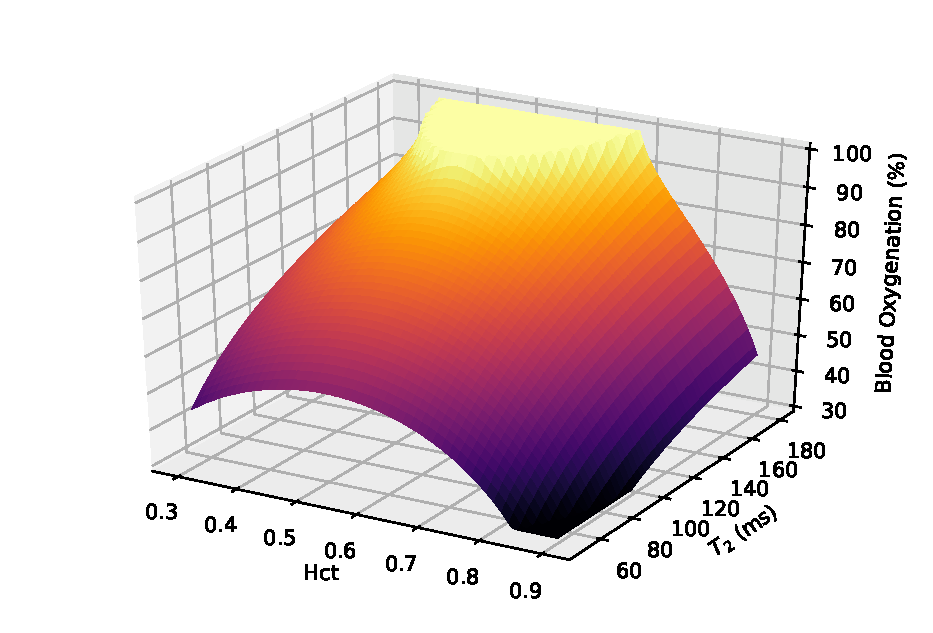
\includegraphics[width=0.7\textwidth]{TRUST/Empirical_surf.eps}
	\caption{The calibration curve used to convert between $T_2$ and $Y_v$ for a given haematocrit \cite{lu_calibration_2012}.}
	\label{fig:calibration_curve}	
\end{figure}

The parameters used in the brain \ac{TILT} \ac{TRUST} sequence were as follows: label slab thickness = 100 mm, imaging slice thickness = 5 mm, distance between centre of imaging slice and centre of labelling slice = 75 mm, \ac{FOV} = 220$\times$220$\times$5 mm, matrix size = 64$\times$64, voxel size = 3.44 $\times$ 3.44 mm, \ac{SENSE} = 3, \ac{EPI} factor = 15, $T_1$ = 1624 ms, \ac{PLD} = 1022 ms, the choice of this value will be explored later, \ac{TR} = 3000 ms, \ac{TE} = 2.9 ms, \ac{eTE} = 1 ms, 40 ms, 80 ms and 160 ms with three pairs of images acquired at each. This led to a total scan duration of approximately 84 seconds.\\

\begin{figure}[H]
	\centering
	\begin{subfigure}[c]{1\textwidth}
		\centering
		\includegraphics[width=1\textwidth]{TRUST/TRUST_FAIR.eps}
		%\missingfigure{TRUST FAIR Seq}
		\caption{}
		\label{fig:TRUST_FAIR_Seq}
	\end{subfigure}
	\vskip\baselineskip
	\begin{subfigure}[c]{0.8\textwidth}
		\centering
		\begin{subfigure}[c]{0.47\textwidth}
			\centering
			\includegraphics[width=1\textwidth]{TRUST/TRUST_FAIR_Brain.eps}
			\caption{}
			\label{fig:TRUST_Brain_FAIR}
		\end{subfigure}
		\hfill
		\begin{subfigure}[c]{0.47\textwidth}
			\centering
			\includegraphics[width=1\textwidth]{TRUST/TRUST_FAIR_Kidney.eps}
			\caption{}
			\label{fig:TRUST_Kidney}
		\end{subfigure}
	\end{subfigure}
	\caption{(\subref{fig:TRUST_FAIR_Seq}) The pulse sequence for \ac{TRUST} \ac{MRI} using the FAIR labelling sequence. (\subref{fig:TRUST_Brain_FAIR}) The selective and non-selective volumes used for tagging via FAIR in the brain. (\subref{fig:TRUST_Kidney}) The selective and non-selective volumes used for tagging via FAIR in the kidneys.}
	\label{fig:TRUST_FAIR}
\end{figure}

The main hurdle to be overcome when moving \ac{TRUST} to the body is the inhomogeneity in the magnetic field caused by the far less homogeneous tissue susceptibilities within the body compared to the brain. These inhomogeneities mean that it is not possible to use \ac{TILT} as the labelling method, instead the  \ac{FAIR} labelling scheme will be used \cite{martirosian_fair_2004}, a diagram of this pulse sequence is shown in Figure \ref{fig:TRUST_FAIR_Seq}. In the \ac{FAIR} labelling scheme a selective inversion pulse is applied with slice selective gradients turned on followed by $T_2$ preparation and acquisition to generate the first image in the pair, a non-selective inversion pulse is then applied with a lower slice selective gradient followed by $T_2$ preparation and then acquisition to generate the second image. An example of the raw images produced is shown in Figure \ref{fig:RV_labsub}. A schematic of the selective and non-selective slices in the brain and the renal vein are shown in Figures \ref{fig:TRUST_Brain_FAIR} and \ref{fig:TRUST_Kidney} respectively. This sequence also has the advantage of being far easier to plan, in the brain having a separate labelling and imaging slice is relatively trivial however the flow of blood in the body is far less ordered and as such, the use of a selective slab within a non-selective slab yields far better results. Movement is a much greater problem in the body. Given the long acquisition time of \ac{TRUST} it is impossible to carry out the scan in a breath hold, as such the sequence is respiratory triggered via a respiratory belt applied around the subjects chest. The total scan time is therefore dependent upon respiratory rate. Depending on the subject, a delay can be applied between the respiratory trigger and the labelling pulse to acquire images while the subject has fully exhaled.\\

\begin{figure}[H]
	\centering
	\begin{subfigure}[c]{0.30\textwidth}
		\centering
		\includegraphics[width=1\textwidth]{TRUST/Kidney_Non_Selective}
		\caption{}
		\label{fig:RV_nonsel}
	\end{subfigure}
	\hfill
	\begin{subfigure}[c]{0.30\textwidth}
		\centering
		\includegraphics[width=1\textwidth]{TRUST/Kidney_Selective}
		\caption{}
		\label{fig:RV_sel}
	\end{subfigure}
	\hfill
	\begin{subfigure}[c]{0.30\textwidth}
		\centering
		\includegraphics[width=1\textwidth]{TRUST/Kidney_eTE_1}
		\caption{}
		\label{fig:RV_diff}
	\end{subfigure}
	\caption{The raw images generated when using the \ac{FAIR} labelling sequence on the kidneys. The non-selective image, (\subref{fig:RV_nonsel}), is subtracted from the selective image, (\subref{fig:RV_sel}), and generates (\subref{fig:RV_diff}), an image of only the untagged blood. The raw \ac{FAIR} images from the brain are omitted as they are very similar to those seen in Figure \ref{fig:SS_labsub}.}
	\label{fig:RV_labsub}
\end{figure}

When using the \ac{FAIR} labelling sequence on the brain the following parameters were used: selective slab thickness = 25 mm, non-selective slab thickness = 400 mm, \ac{FOV} = 220$\times$220$\times$5 mm, matrix size = 64$\times$64, voxel size = 3.44 $\times$ 3.44 $\times$ 5 mm, \ac{SENSE} = 3, \ac{EPI} factor = 15, $T_1$ = 1624 ms, \ac{PLD} = 800 ms, \ac{TR} = 7276 ms, \ac{TE} = 2.9 ms, \ac{eTE} = 1 ms, 40 ms, 80 ms and 160 ms with three pairs of images acquired at each. When used on the body, the parameters were as follows: selective slab thickness = 25 mm, non-selective slab thickness = 400 mm, \ac{FOV} = 244$\times$244$\times$5 mm, matrix size = 96$\times$96, voxel size = 3.44 $\times$ 3.44 $\times$ 5 mm, \ac{SENSE} = 3, \ac{EPI} factor = 15, $T_1$ = 1624 ms, \ac{PLD} = 1000 ms, the choice of this value will be explored later, \ac{TR} = 8076 ms, \ac{TE} = 2.9 ms, \ac{eTE} = 1 ms, 40 ms, 80 ms and 160 ms with three pairs of images acquired at each.\\

\subsubsection{Analysis}
\label{sec:trust_analysis}
The analysis of the data collected using the above protocol was carried out using custom \textsc{MATLAB} (MathWorks, Natick, MA) software based upon code written by Liu and modified to work with data collected using the \ac{FAIR} labelling method by Cox \cite{liu_pro_2011}. This software loads the data and carries out the subtraction of each image pair then presents a difference image to the user so the vessel can be drawn around. At this point the voxels with the greatest intensity within the vessel, four voxels when calculating $Y_v$ for the superior sagittal sinus and nine voxels when working on the renal vein, are averaged, as are the intensities of each repeat \ac{eTE}. These mean signals are then fit to Equation \eqref{eq:TRUST} to compute a value of $T_2$ with confidence bounds. The value of $Y_v$ can then be found using the aforementioned calibration curve. Once the software has finished, it saves all outputs and intermediary variables to a file on the computer for later analysis.

\subsection{Inducing Changes in Oxygenation of Blood in the Renal Vein}

In order to assess the ability of these methods to measure a change in renal oxygenation, a method of inducing such a change in the kidneys needed to be devised. Looking at literature that has carried out similar studies, it is suggested that changes in renal oxygenation can be induced by either varying the subjects sodium intake, water intake or inspired oxygen level \cite{oconnor_comparison_2009, donati_quantitative_2012}.\\

Due to the challenges associated with controlling subjects diet for two weeks as was performed in Priijm \cite{pruijm_effect_2010}, the use of sodium intake was discounted. From previous work we know that applying a large water load to subjects during the scanning session, as in Tumkur and Prasad  \cite{tumkur_evaluation_2006, prasad_changes_1999}, can cause undesired effects on the resultant shim as assessed by $B_0$ maps due to the large susceptibility change adding such a large quantity of water to the abdomen can cause, as such, this method was also discounted leaving us to pursue an oxygen challenge.\\

This method consisted of localisers and anatomical images being collected followed by alternating \ac{BOLD} $T_2^*$ and \ac{TRUST} scans while the subject was breathing room air to record a baseline. Pure oxygen was then delivered to the subject at 15 $\ell$/min via a gas mask and, after a two minute wash in period, the \ac{BOLD} $T_2^*$ and \ac{TRUST} scans were repeated. A visual representation of this protocol can be seen in Figure \ref{fig:oxygen_challenge_protocol}. The \ac{BOLD} $T_2^*$ scans had a slice thickens of 5 mm, 12 echoes with an initial \ac{TE} of 5 ms and subsequent echo spacing of 3 ms, the flip angle was $30\degree$. The total scan time was approximately 17 seconds and was acquired during a single breath hold. The \ac{TRUST} scans were conducted as per Section \ref{sec:TRUST_MRI}.\\

\begin{figure}[H]
	\centering
	\includegraphics[width=0.95\textwidth]{TRUST/Protocol.eps}
	\caption{The protocol used to induce changes in renal oxygenation.}
	\label{fig:oxygen_challenge_protocol}	
\end{figure}

\newpage
\section{Results and Discussion}
\subsection{Susceptibility-Based Oximetry}
\subsubsection{Susceptibility-Based Oximetry in the Brain}

Having collected data using the method outlined in \ref{sec:SBO_prot} it was possible to use Equation \eqref{eq:SBO} to estimate $Y_v$ in the superior sagittal sinus to be $63\pm2.1\%$. This is consistent with the value reported by Liu of $61.1\pm1.4\%$ found in a multi centre \ac{TRUST} trial with 250 participants over a wide range of ages and ethnicity distribution \cite{liu_multi-site_2016}.

\subsubsection{Susceptibility-Based Oximetry in the Renal Vein}
Having calculated an acceptable result in the brain that agreed with literature it was possible to move onto applying techniques to assess oxygenation in the renal vein. A set of three phase maps were collected along with three localisers, one along each plane. If $\Delta \phi$ is plot against $\theta$ for a typical $Y_v$ of 85\%, Figure \ref{fig:SBO_kidney} is produced. It can be seen that, for an expected $Y_v$, the phase difference is greatest if the vessel runs parallel to the $B_0$ field. No part of the renal vein is located parallel to the $B_0$ field, typically the angle is in the region of $75\degree$ (there is a large degree of variability in vasculature geometry between subjects) and as such delivers a very small phase difference. This coupled with the fact that the gradient of this function at these angles is large, meaning that the uncertainty in angle corresponds to a larger uncertainty in $Y_v$ means it will unfortunately not be possible to use susceptibility-based oximetry to accurately measure $Y_v$ within the renal vein.\\

\begin{figure}[H]
	\centering
	\includegraphics[width=0.60\textwidth]{TRUST/SBO_angle.eps}
	\caption{For a typical $Y_v$ of 85\% the phase difference produced by a vessel at a range of angles to $B_0$.}
	\label{fig:SBO_kidney}	
\end{figure}
This technique would perhaps be better suited to use in the liver to assess oxygenation in the portal vein. This vessel runs at a much smaller angle to the $B_0$ field and as such the model will still be valid with reasonable errors, Figure \ref{fig:PV}. This would potentially work much better than \ac{TRUST} here as the sequence is much quicker and therefore will be less susceptible to movement.

\begin{figure}[H]
	\centering
	\includegraphics[width=0.5\textwidth]{TRUST/Organ_Schematic_Both-01.eps}
	\caption{A schematic of the portal and renal veins entering the liver and left kidney respectively in relation to the $B_0$ field.}
	\label{fig:PV}	
\end{figure}

\subsection{$T_2$ Relaxation Under Spin Tagging}
\subsubsection{\ac{TRUST} in the Brain}

To test if the \ac{FAIR} labelling sequence delivered the same signal decay as the \ac{TILT} sequence both labelling schemes were performed sequentially on the superior sagittal sinus with a \ac{PLD} of 800 ms. The resulting normalised signals are shown in Figure \ref{fig:TILT_vs_FAIR}.
\begin{figure}[H]
	\centering
	%\missingfigure{T2 curves for TILT and FAIR}
	\includegraphics[width=0.55\textwidth]{TRUST/TILT_vs_FAIR.eps}
	\caption{The signal decay within the superior sagittal sinus found using \ac{TRUST} with both \ac{TILT} and \ac{FAIR} labelling sequences scaled by their initial signal intensities at eTE = 1 ms.}
	\label{fig:TILT_vs_FAIR}	
\end{figure}

As can be seen these signals are in excellent agreement with the \ac{TILT} sequence producing a $T_2$ of $52\pm1$ ms and the \ac{FAIR} sequence producing a $T_2$ of $50\pm2$ ms, therefore in agreement within the bounds of error. This means that \ac{FAIR} can be directly substituted for \ac{TILT} in the \ac{TRUST} sequence to measure $Y_v$ in the superior sagittal sinus and can subsequently be used for the renal \ac{TRUST} measurements.\\

To find the dependence \ac{PLD} has upon the signal measured, scans were carried out at a range of delays from 400 ms to 1400 ms while using the \ac{FAIR} labelling sequence. The signal from \ac{eTE}=1 ms was then plot against label delay. Figure \ref{fig:Sig_vs_PLD_SS} shows the signal from the difference images. The maximum signal is observed with a \ac{PLD} of 800 ms. This value is reached due to the balance between $T_1$ relaxation of the non-selective blood and inflow of unlabelled blood. This maximum in signal agrees with literature using the \ac{TILT} labelling scheme \cite{lu_quantitative_2008}. By carrying out scans with this \ac{PLD} the maximum \ac{SNR} will be achieved.\\ 

\begin{figure}[H]
	\centering
	\includegraphics[width=0.55\textwidth]{TRUST/PLD_SS.eps}
	\caption{The mean signal from the first echo of each difference image over a range of \ac{PLD} times.}
	\label{fig:Sig_vs_PLD_SS}	
\end{figure}

$T_2$ should have no dependence upon \ac{PLD} given the signal from the difference image will have the same decay in time, it will just be a lower intensity for non-optimal \ac{PLD} thus leading to a larger confidence interval. To confirm this the fit values of $T_2$ were plot against \ac{PLD}, Figure \ref{fig:SS_T2vsPLD}.

\begin{figure}[H]
	\centering
	\includegraphics[width=0.55\textwidth]{TRUST/T2_vs_PLD_SS.eps}
	\caption{The dependence of $T_2$ upon \ac{PLD}.}
	\label{fig:SS_T2vsPLD}	
\end{figure}


It can be seen that, as predicted, there is no relationship between $T_2$ and \ac{PLD}. An increase in error with label delay was not observed, this effect may only show itself at larger values of \ac{PLD} however for our purposes, simply confirming there is no large increase in error around our chosen \ac{PLD} is sufficient. This means that if there is a variation in the optimum \ac{PLD} between subjects due to the larger range in \ac{RBF} compared to \ac{CBF} then this will not have an affect upon the value of $T_2$ and thus $Y_v$.\\

When the analysis is carried out on the images, the four brightest voxels of the difference image are averaged before the fitting occurs. This number of voxels is chosen due to the average size of the superior sagittal sinus however, for some subjects more voxels could be included, potentially yielding better results. To assess the variability in $T_2$ measurements with the number of voxels averaged, the analysis was run multiple times with one to twelve voxels included in the calculation. Multiple \ac{TRUST} scans were performed on the same subject and averaged generating Figure \ref{fig:nvox_SS}.\\

\begin{figure}[H]
	\centering
	\begin{subfigure}[c]{0.47\textwidth}
		\centering
		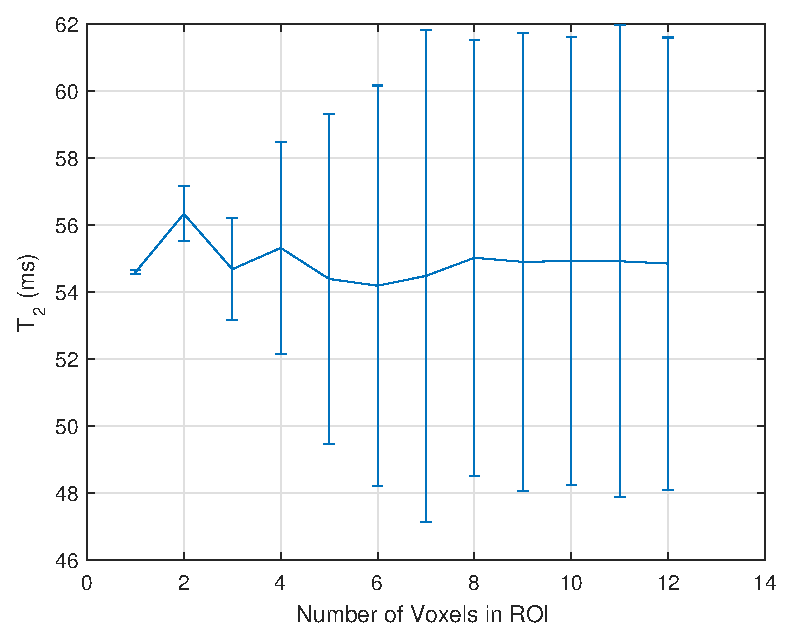
\includegraphics[width=0.9\textwidth]{TRUST/SS_T2_vs_nvox_mean2.eps}
		\caption{}
		\label{fig:nvox_SS}
	\end{subfigure}
	\hfill
	\begin{subfigure}[c]{0.47\textwidth}
		\centering
		\includegraphics[width=.7\textwidth]{TRUST/SS_ROI}
		\caption{}
		\label{fig:SS_ROI}
	\end{subfigure}
	\caption{(\subref{fig:nvox_SS}) The value of $T_2$ computed for the superior sagittal sinus with different numbers of voxels included in the calculation. (\subref{fig:SS_ROI}) The difference image of the superior sagittal sinus with a three voxel \ac{ROI} shown. This is already covering most of the vessel, hence the noise going up as more voxels are added to the calculation.}
	\label{fig:nv_SS}
\end{figure}

Although from Figure \ref{fig:nvox_SS} it would appear that it would be best to only use the brightest voxel in the calculation due to its very small error and that it has the same value of $T_2$ as the results with far more voxels; this would not be a very robust method. It is fairly easy to conceive a greater than average level of noise being recorded on a single pixel in the relaxation and as such skewing the output of the calculation. The confidence interval is so large above six voxels because by this point the calculations are simply including the noise around the vessel rather than the signal from the blood within the sagittal sinus. Given these results, using four voxels in the calculation seems to be a reasonable balance between uncertainty and robustness.\\

To assess the repeatability of this measure, the optimised scan was repeated ten times on a single subject during one scanning session. This yielded a $Y_v$ of $69.5\pm0.6$\%, a value consistent with literature \cite{nagdyman_comparison_2005, liu_multi-site_2016}. Given the success of the modified sequence on the superior sagittal sinus, it was possible to attempt to measure $Y_v$ in the renal vein.\\

\subsubsection{\ac{TRUST} in the Body}

Ideal vessels to test the \ac{TRUST} sequence within the body are the portal vein and hepatic artery as these vessels are large, have different oxygen saturations and can easily be imaged at the same time. Using the modified \ac{TRUST} sequence the $T_2$ and oxygen saturation of the portal vein was found to be 109 $\pm$ 5 ms and 79.9 $\pm$ 0.8 \% respectively; the $T_2$ and oxygen saturation of the hepatic artery was found to be 157 $\pm$ 10 ms and 100 $\pm$ 1 \% respectively. This means that, as expected, the oxygen saturation in the hepatic artery is measured as greater than that of the portal vein and therefore the \ac{TRUST} protocol is working as expected. Although normally the analysis would simply be based upon the mean of the brightest voxels in the difference image as outlined in Section \ref{sec:trust_analysis}, in Figure \ref{fig:pv_TRUST} a voxel by voxel analysis has been carried out for illustrative purposes.\\

\begin{figure}[h]
	\centering
	\includegraphics[width=0.5\textwidth]{TRUST/PV_TRUSTmap.eps}
	\caption{The oxygen saturation of the portal vein and hepatic artery measured using \ac{TRUST}.}
	\label{fig:pv_TRUST}	
\end{figure}
To assess if the \ac{PLD} that generates the greatest signal is the same in the renal vein as in the superior sagittal sinus, a series of scans were collected with \ac{PLD} ranging from 400 ms to 1400 ms and the signal from \ac{eTE} = 1 ms recorded.\\
%\begin{figure}[H]
%	\centering
%	\includegraphics[width=0.65\textwidth]{Signal_vs_Label_Delay_RV.eps}
%	\caption{The mean signal from the first echo of each difference image of the renal vein over a range of \ac{PLD}}
%	\label{fig:Sig_vs_PLD_RV}	
%\end{figure}

\begin{figure}[H]
	\centering
	\begin{subfigure}[c]{0.47\textwidth}
		\centering
		\includegraphics[width=1\textwidth]{TRUST/PLD_RV.eps}
		\caption{}
		\label{fig:Sig_vs_PLD_RV}
	\end{subfigure}
	\hfill
	\begin{subfigure}[c]{0.47\textwidth}
		\centering
		\includegraphics[width=1\textwidth]{TRUST/PLD_RV_More_Data.eps}
		\caption{}
		\label{fig:Sig_vs_PLD_RV_more}
	\end{subfigure}
	\caption{(\subref{fig:Sig_vs_PLD_RV}) The mean signal from the first echo of each difference image of the renal vein over a range of \ac{PLD}. (\subref{fig:Sig_vs_PLD_RV_more}) Mean signal from the first echo versus \ac{PLD} from a different subject. }
\end{figure}

As seen in Figure \ref{fig:Sig_vs_PLD_RV} the \ac{PLD} producing the largest signal in the difference image of the renal vein is indeed different to that of the superior sagittal sinus. This is most likely due to differences in blood flow through each of these vessels, $413\pm136$ ml/min in the renal vein \cite{cox_multiparametric_2017} and $285\pm19$ ml/min in the superior sagittal sinus \cite{jordan_velocity_1994}. Given the much larger uncertainty in blood flow in the renal vein, a different subject was scanned over a smaller range of \ac{PLD} to ascertain if the \ac{PLD} delivering the maximum signal varies much between subjects, Figure \ref{fig:Sig_vs_PLD_RV_more}.\\

The maximum signal for the first subject was achieved at a \ac{PLD} of 1200 ms whereas for the second subject the maximum is at a \ac{PLD} of 800 ms. Given that these subjects had a \ac{RBF} either side of the mean and that there is little dependence of $T_2$ upon \ac{PLD} it seems appropriate to use a \ac{PLD} of 1000 ms for optimum signal in most subjects.\\

Given the larger size of the renal vein compared to the superior sagittal sinus, it would be better to include more voxels in the calculations when fitting to find a value of $T_2$. Multiple scans were completed on a single subject and the value of $T_2$ found for each using one to twelve voxels in the fitting process. The results were averaged and plot in Figure \ref{fig:nvox_RV}.\\

\begin{figure}[H]
	\centering
	\begin{subfigure}[c]{0.47\textwidth}
		\centering
		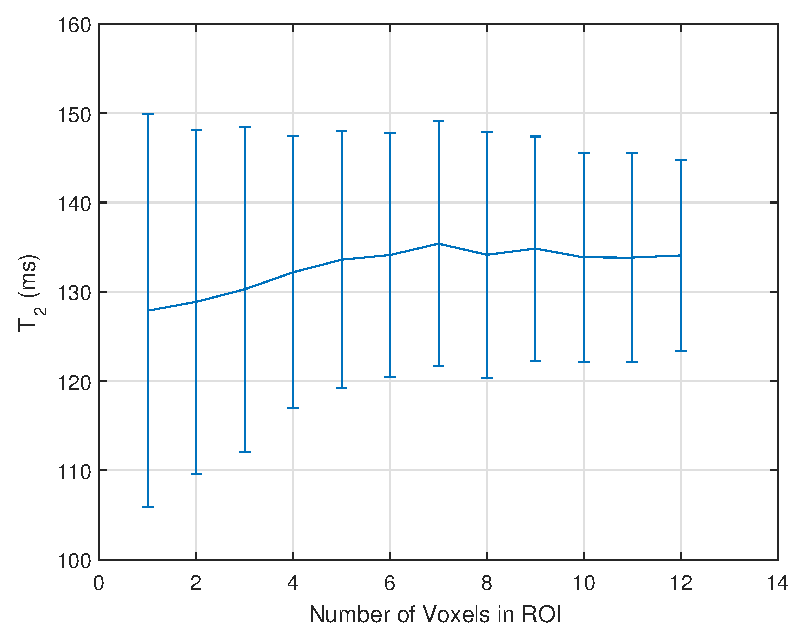
\includegraphics[width=1\textwidth]{TRUST/RV_T2_vs_nvox_mean_S2.eps}
		\caption{}
		\label{fig:nvox_RV}
	\end{subfigure}
	\hfill
	\begin{subfigure}[c]{0.47\textwidth}
		\centering
		\includegraphics[width=.7\textwidth]{TRUST/RV_ROI}
		\caption{}
		\label{fig:RV_ROI}
	\end{subfigure}
	\caption{(\subref{fig:nvox_RV}) The value of $T_2$ calculated for the renal vein with different numbers of voxels included in the calculation. (\subref{fig:RV_ROI}) The difference image of the renal vein with a nine voxel \ac{ROI} shown.}
	\label{fig:nv_RV}
\end{figure}


Unlike the results when this process was carried out on the superior sagittal sinus in Figure \ref{fig:nvox_SS}, here the error decreases as more voxels are added to the calculation. This uncertainty comes from the large variation in $T_2$ for one voxel rather than a large error on the fit i.e. the error is coming from the differences between scans rather than the robustness of each scans results, this is precisely the concern that was raised with using a single voxel when discussing the superior sagittal sinus. As more voxels are added the error decreases until approximately six voxels are included, at this point the value of $T_2$ stops increasing and stays approximately constant. Once again, given the large variation in renal veins, it would be advisable to include slightly more than six voxels but not so many that in the cases of small vessels the algorithm is sampling surrounding tissue. Nine voxels seems to be a suitable middle ground as to work effectively with both small and large vessels.\\

To assess the repeatability of the measurements within the kidney, the same scan was repeated ten times in a single session with the optimised renal parameters. This yielded a $T_2$ of $135\pm5$ ms corresponding to a $Y_v$ of $89\pm2\%$. The variation in measurements of $Y_v$ in the renal vein are relatively substantial and show no dependence upon time so are therefore not likely due to physiological changes. The value of $Y_v$ in the renal vein is much higher than in the sagittal sinus however is within the range found by Nielsen \cite{nielsen_renal_1992}.\\

\begin{figure}[H]
	\centering
	\includegraphics[width=0.55\textwidth]{TRUST/T2_Decay_Body.eps}
	\caption{The $T_2$ relaxation curves of ten scans repeated on a single subject.}
	\label{fig:T2_Decay_Body}	
\end{figure}

To compare the abilities of \ac{BOLD} $T_2^*$ maps and \ac{TRUST} to measure changes in oxygenation in the kidneys, a hyperoxia challenge was conducted. In Figure \ref{fig:dT2star}, no systematic, bulk change in $T_2^*$ can be seen indicating that the change in $T_2^*$ caused by the introduction of pure oxygen is dominated by other confounding factors. This is confirmed when \ac{ROI} are defined for the renal cortex and renal medulla with the mean change in $T_2^*$ found to be $-2 \pm 8$ ms and $-1 \pm 6$ ms respectively. When \ac{TRUST} is used to measure the oxygen saturation in the renal vein an increase of 16 $\pm$ 3 \% is observed, Figure \ref{fig:dYv}. This shows that it is possible to measure changes in renal oxygenation using \ac{TRUST} that would be undetectable using the current standard, \ac{BOLD} $T_2^*$ mapping.
\begin{figure}[H]
	\centering
	\begin{subfigure}[c]{0.47\textwidth}
		\centering
		\includegraphics[width=1\textwidth]{TRUST/dT2star_M0.eps}
		\caption{}
		\label{fig:dT2star}
	\end{subfigure}
	\hfill
	\begin{subfigure}[c]{0.47\textwidth}
		\centering
		\includegraphics[width=1\textwidth]{TRUST/dYv_Sub_2.eps}
		\caption{}
		\label{fig:dYv}
	\end{subfigure}
	\caption{(\subref{fig:dT2star}), The difference in $T_2^*$ measured between baseline and the hyperoxia state. (\subref{fig:dYv}) The difference in $Y_v$ measured using \ac{TRUST}.}
	\label{fig:oxygen_chalenge_results}
\end{figure}

\newpage
\section{Conclusions and Future Work}

This work shows promising results for the use of a modified \ac{TRUST} sequence to measure oxygenation of blood within the body. The existing \ac{TRUST} sequence was modified to be respiratory triggered and use the \ac{FAIR} labelling scheme making it suitable for use in the body. Once these modifications had been carried out, parameters such as \ac{PLD} and the number of voxels used in the \ac{ROI} were optimised. The ability of \ac{TRUST} to measure a change in renal oxygenation was successfully verified via a hyperoxia challenge which was able to measure an increase of 16 $\pm$ 3 \% where the current standard measurement of renal oxygenation, \ac{BOLD} $T_2^*$ maps, recorded no significant change.\\

Looking forward this work could be expanded by carrying out the hyperoxia challenge on more subjects. Although a small number of measurements were gathered on the hepatic vessels, further work could be undertaken to compare the use of susceptibility based oximetry and \ac{TRUST} to measure oxygenation in the portal vein in response to a hyperoxia challenge as conducted for the kidneys here. In the current protocol, haematocrit is assumed to be an average value of 0.41 unless a blood test has recently been undertaken. As stated above, there is a correlation between $T_1$ of blood and its haematocrit, this means that a measurement of the subjects haematocrit could be taken while they are in the scanner, thus leading to a more accurate measurement of oxygenation with only a small increase in scan time. 

\section{Acknowledgements}

We thank Hanzhang Lu for sharing the TRUST methodology.\\
